\documentclass[10pt]{article}

% ============================================================
% PACKAGES
% ============================================================

\usepackage[a4paper,margin=0.65in]{geometry}
\usepackage{amsmath,amssymb}
\usepackage{graphicx}
\usepackage{booktabs}
\usepackage{array}
\usepackage{float}
\usepackage{hyperref}
\usepackage{enumitem}
\usepackage{xcolor}
\usepackage{tikz}
\usepackage{multirow}
\usepackage{caption}
\usepackage{subcaption}

\usetikzlibrary{
positioning,
arrows.meta,
shapes.geometric,
fit,
calc
}

% ============================================================
% FORMATTING
% ============================================================

\setlist{nosep,leftmargin=*}
\renewcommand{\arraystretch}{1.2}
\setlength{\parindent}{0pt}
\setlength{\parskip}{2pt}
\setlength{\emergencystretch}{3em}

\hypersetup{
    colorlinks=true,
    linkcolor=blue,
    urlcolor=blue,
    citecolor=blue
}

% ============================================================
% TIKZ STYLES
% ============================================================

\tikzset{
block/.style={
draw,
rounded corners,
minimum width=1.55cm,
minimum height=0.60cm,
align=center,
fill=blue!10,
font=\scriptsize
},
attn/.style={
draw,
rounded corners,
minimum width=1.55cm,
minimum height=0.60cm,
align=center,
fill=green!12,
font=\scriptsize
},
arrow/.style={
-{Latex[length=2mm]},
thin
}
}

% ============================================================
% DOCUMENT
% ============================================================

\begin{document}

% ============================================================
% TITLE
% ============================================================

\begin{center}

{\large\textbf{Shiv Nadar University Chennai}}\\[2mm]

{\normalsize\textbf{CS3807 -- Deep Learning Laboratory}}\\[2mm]

{\large\textbf{Experiments 8, 9}}\\[1mm]

{\normalsize
\textbf{
Effect of Attention Type and Attention Position\\
in a Pretrained ResNet50
}}

\end{center}

\begin{flushleft}
\textbf{Name:} Johan Emmanuel S\\
\textbf{Registration Number:} 24011101043\\
\end{flushleft}

\vspace{3mm}

% ============================================================
% COURSE DETAILS
% ============================================================

\begin{center}
\begin{tabular}{|p{3.5cm}|p{8.7cm}|p{2.1cm}|}
\hline
\textbf{Degree \& Branch}
&
B.Tech Artificial Intelligence \& Data Science
&
Semester V
\\
\hline

\textbf{Subject Code \& Name}
&
CS3807 -- Deep Learning Laboratory
&
AY: 2026--27
\\
\hline
\end{tabular}
\end{center}

% ============================================================
\section*{1. Aim}
% ============================================================

The aim of this experiment is to study how different attention mechanisms
modify a pretrained convolutional neural network and how the
\textbf{position at which attention is inserted} influences image
classification performance.

A single pretrained architecture,

\[
\boxed{\text{ResNet50 pretrained on ImageNet}}
\]

is used throughout the experiment. The following were investigated on the
five-class flower dataset:

\begin{itemize}
\item channel attention, spatial attention, sequential channel--spatial attention and lightweight self-attention;
\item four insertion positions within ResNet50, and single-stage versus multi-stage attention;
\item attention ordering and the spatial-attention kernel size;
\item additional established mechanisms (ECA, CBAM, Coordinate Attention); and
\item qualitative interpretation using internal attention maps and Grad-CAM.
\end{itemize}

The effectiveness of attention depends not only on the attention mechanism
itself, but also on the characteristics of the feature representation on
which it operates.

% ============================================================
\section*{2. Dataset Description}
% ============================================================

\textbf{TensorFlow Flowers (\texttt{tf\_flowers})} contains $3{,}670$ natural
RGB flower images belonging to five classes: \texttt{dandelion} (898 images),
\texttt{daisy} (633), \texttt{tulips} (799), \texttt{sunflowers} (699) and
\texttt{roses} (641). The images contain variations in scale, viewpoint,
illumination, background clutter, flower size, color, texture and object
location, which makes the dataset suitable for studying attention.

% ============================================================
\subsection*{2.1 Image Preprocessing}
% ============================================================

Every image was resized to

\[
224\times224\times3
\]

and preprocessed using the preprocessing function of the ImageNet-pretrained
ResNet50. Data augmentation (training set only) consisted of random
horizontal flipping, random rotation (factor $0.05$, approximately
$\pm18^\circ$), random zoom ($0.10$), random translation ($0.10$ in both
directions) and random contrast ($0.10$). The same augmentation strategy was
used for every model.

\begin{figure}[H]
\centering
\includegraphics[width=0.78\linewidth]{01_samples.eps}
\caption{Sample training images (six per class) from all five classes.}
\end{figure}

\begin{figure}[H]
\centering
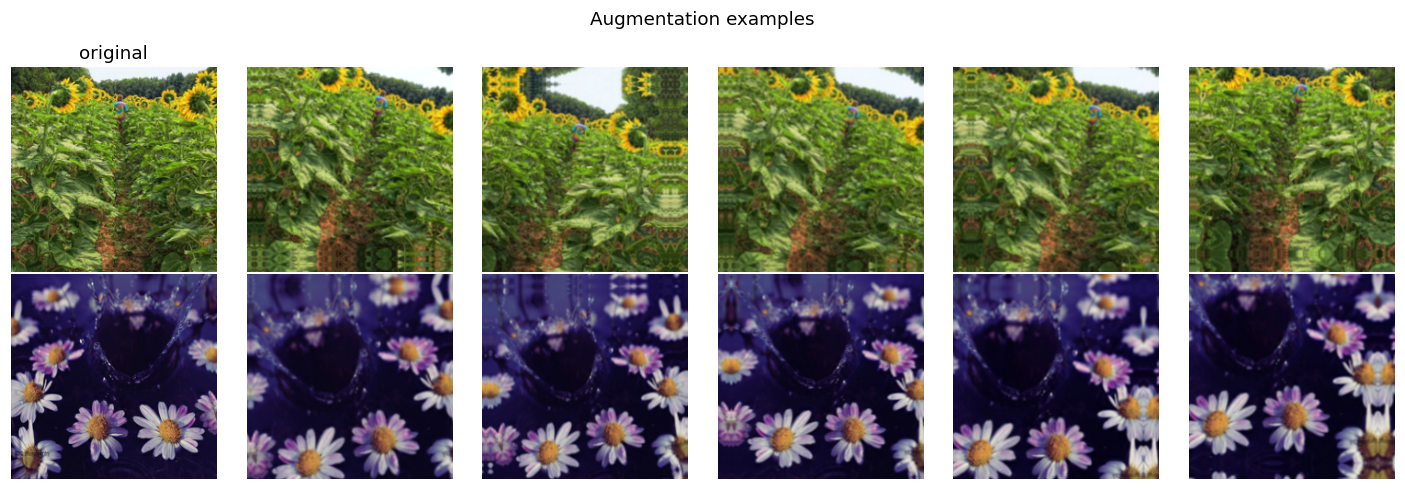
\includegraphics[width=0.9\linewidth]{02_augmentation.png}
\caption{Augmentation examples (first column: original image).}
\end{figure}

% ============================================================
\subsection*{2.2 Dataset Split}
% ============================================================

A stratified split was fixed once (seed $42$) and reused for every experiment:

\[
\boxed{
70\% : 15\% : 15\%
}
\quad\Rightarrow\quad
2569 : 550 : 551
\]

for Training : Validation : Testing. The train, validation and test index
sets were verified to be mutually disjoint. The test set contains 135
\texttt{dandelion}, 95 \texttt{daisy}, 120 \texttt{tulips}, 105
\texttt{sunflowers} and 96 \texttt{roses} images.

% ============================================================
\section*{3. ResNet50 Architecture}
% ============================================================

ResNet50 pretrained using ImageNet is used as the
\textbf{only backbone architecture}. For an input image
$I\in\mathbb{R}^{224\times224\times3}$, the major ResNet50 stages produce
the following feature dimensions:

\begin{center}

\begin{tabular}{|l|c|c|}
\hline
\textbf{ResNet50 Stage}
&
\textbf{Spatial Resolution}
&
\textbf{Channels}
\\
\hline

Stem + MaxPool
&
$56\times56$
&
64
\\
\hline

conv2\_x
&
$56\times56$
&
256
\\
\hline

conv3\_x
&
$28\times28$
&
512
\\
\hline

conv4\_x
&
$14\times14$
&
1024
\\
\hline

conv5\_x
&
$7\times7$
&
2048
\\
\hline

\end{tabular}

\end{center}

As the network becomes deeper, the spatial resolution decreases while the
number of feature channels increases, and the representation progresses from
low-level visual information toward high-level semantic information:

\begin{itemize}
\item \textbf{Early features:} edges, colors, orientations, boundaries and simple textures.
\item \textbf{Intermediate features:} local patterns, repeated structures, flower parts, petal arrangements and shape information.
\item \textbf{Late features:} high-level object structures and class-discriminative semantic information.
\end{itemize}

Attention is not independent of the features on which it operates: early-stage
attention acts on high-resolution, low-level information, middle-stage
attention on intermediate features, and late-stage attention on
low-resolution, high-level semantic representations. Four candidate
attention positions were therefore defined: $P_1$ after conv2\_x, $P_2$
after conv3\_x, $P_3$ after conv4\_x and $P_4$ after conv5\_x. The last two
columns of the table give the size of the $N\times N$ self-attention matrix
($N=HW$) that would be produced at each position (single image, fp32).

\begin{center}

\begin{tabular}{|c|c|c|c|c|c|}
\hline

\textbf{Position}
&
\textbf{Location}
&
\textbf{Resolution}
&
\textbf{Channels}
&
\textbf{$N=HW$}
&
\textbf{$N\times N$ entries (MB)}
\\
\hline

$P_1$
&
After conv2\_x
&
$56\times56$
&
256
&
3136
&
9,834,496 (37.52)
\\
\hline

$P_2$
&
After conv3\_x
&
$28\times28$
&
512
&
784
&
614,656 (2.34)
\\
\hline

$P_3$
&
After conv4\_x
&
$14\times14$
&
1024
&
196
&
38,416 (0.15)
\\
\hline

$P_4$
&
After conv5\_x
&
$7\times7$
&
2048
&
49
&
2,401 (0.01)
\\
\hline

\end{tabular}

\end{center}

The self-attention matrix grows with the square of the number of spatial
positions, from 2,401 entries at $P_4$ to almost 9.8 million entries at
$P_1$ (a factor of about 4096).

% ============================================================
\section*{4. Attention Mechanisms}
% ============================================================

\subsection*{4.1 Channel Attention}

For a feature tensor $F\in\mathbb{R}^{H\times W\times C}$, global average
pooling gives the channel descriptor
\[
z_c
=
\frac{1}{HW}
\sum_{i=1}^{H}
\sum_{j=1}^{W}
F(i,j,c),
\]
which is transformed by two learnable layers:
\[
M_c(F)
=
\sigma
\left(
W_2
\delta
\left(
W_1z
\right)
\right),
\qquad
F_c
=
F\odot M_c(F),
\]
where $\delta(\cdot)$ is ReLU, $\sigma(\cdot)$ is the sigmoid, $W_1$ reduces
and $W_2$ restores the channel dimension. A reduction ratio $r=16$ was used
throughout (not ablated). This block is identical to a Squeeze-and-Excitation
(SE) block, so ``Channel'' and ``SE'' denote the same model. Channel
attention answers: \emph{which feature channels are important?}

\subsection*{4.2 Spatial Attention}

Average and maximum pooling across channels give
$F_{\mathrm{avg}}=\operatorname{Mean}_c(F)$ and
$F_{\mathrm{max}}=\operatorname{Max}_c(F)$, both of size $H\times W\times1$.
After concatenation, $F_s=[F_{\mathrm{avg}}\Vert F_{\mathrm{max}}]$,
\[
M_s(F)
=
\sigma
\left(
\operatorname{Conv}_{k\times k}(F_s)
\right)
\in\mathbb{R}^{H\times W\times1},
\qquad
F_s'
=
F\odot M_s(F),
\]
with $k=7$ by default. Spatial attention answers: \emph{which spatial
locations are important?}

\subsection*{4.3 Sequential Channel--Spatial Attention}

\[
F_c=M_c(F)\odot F,
\qquad
F_{cs}=M_s(F_c)\odot F_c,
\]
that is, first ``what is important'' and then ``where it is important''.

\begin{center}

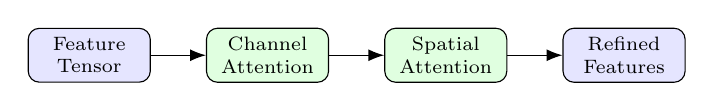
\begin{tikzpicture}[node distance=7mm]

\node[block] (a)
{Feature\\Tensor};

\node[attn,right=of a] (b)
{Channel\\Attention};

\node[attn,right=of b] (c)
{Spatial\\Attention};

\node[block,right=of c] (d)
{Refined\\Features};

\draw[arrow] (a)--(b);
\draw[arrow] (b)--(c);
\draw[arrow] (c)--(d);

\end{tikzpicture}

\end{center}

\subsection*{4.4 Self-Attention}

Flattening the spatial dimensions gives $X\in\mathbb{R}^{N\times C}$ with
$N=HW$. Then $Q=XW_Q$, $K=XW_K$, $V=XW_V$,
\[
A
=
\operatorname{softmax}
\left(
\frac{QK^T}{\sqrt{d}}
\right),
\qquad
Y=AV,
\qquad
F_{\mathrm{SA}}
=
F
+
\gamma
\operatorname{reshape}(Y),
\]
where $\gamma$ is a learnable scalar initialised to zero. The implementation
uses a query/key dimension $d=C/8$ and a value dimension $C/2$.
Self-attention answers: \emph{which spatial features are related to other
spatial features?} Its cost grows with $N^2$ (see Section 3).
The \textbf{Combined} model (A5) applies Channel $\rightarrow$ Spatial
$\rightarrow$ Self-attention in sequence.

\subsection*{4.5 Additional Mechanisms}

\begin{itemize}
\item \textbf{ECA:} a 1-D convolution of adaptive odd kernel size over the pooled channel descriptor, with no dimensionality reduction (kernel size 5 at 1024 channels and 7 at 2048 channels).
\item \textbf{CBAM:} channel attention using both average- and max-pooled descriptors through a shared MLP (summed, then sigmoid), followed by $7\times7$ spatial attention.
\item \textbf{Coordinate Attention (CoordAtt):} direction-aware pooling along height and width, a shared $1\times1$ convolution with batch normalisation and h-swish, and separate sigmoid gates for the two directions (reduction 32).
\end{itemize}

% ============================================================
\section*{5. Proposed Experimental Architecture}
% ============================================================

The baseline is the pretrained ResNet50 without any additional attention
mechanism.

\begin{center}

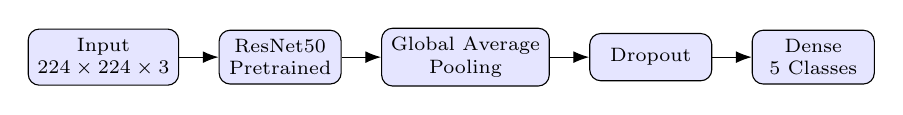
\begin{tikzpicture}[node distance=5mm]

\node[block] (a)
{Input\\$224\times224\times3$};

\node[block,right=of a] (b)
{ResNet50\\Pretrained};

\node[block,right=of b] (c)
{Global Average\\Pooling};

\node[block,right=of c] (d)
{Dropout};

\node[block,right=of d] (e)
{Dense\\5 Classes};

\foreach \x/\y in {a/b,b/c,c/d,d/e}
\draw[arrow] (\x)--(\y);

\end{tikzpicture}

\end{center}

For any selected stage $P_k$, the attention-based network is
\[
\text{Previous ResNet Stage}
\rightarrow
\text{Attention}
\rightarrow
\text{Next ResNet Stage},
\]
for example
$\text{conv4\_x}\rightarrow\text{Channel Attention}\rightarrow\text{Spatial Attention}\rightarrow\text{conv5\_x}$
for channel--spatial attention at $P_3$.

\textbf{Feature dimensions before and after attention.} Every attention
module preserved the tensor shape (verified by an assertion for all 19
attention placements). The dimensions immediately before and after the
attention block were $(56,56,256)\rightarrow(56,56,256)$ at $P_1$,
$(28,28,512)\rightarrow(28,28,512)$ at $P_2$,
$(14,14,1024)\rightarrow(14,14,1024)$ at $P_3$ and
$(7,7,2048)\rightarrow(7,7,2048)$ at $P_4$. Placements verified: Channel/SE,
Spatial, Chan$\rightarrow$Spat, Self-Attn, Combined, Spat$\rightarrow$Chan,
$k=3$, $k=5$, ECA, CBAM and CoordAtt at $P_3$; C$\rightarrow$S at $P_1$,
$P_2$ and $P_4$; C$\rightarrow$S at $P_3{+}P_4$ (both positions) and at
$P_2{+}P_3{+}P_4$ (all three positions).

% ============================================================
\section*{6. Experimental Setup}
% ============================================================

\textbf{Transfer-learning strategy.} ImageNet weights were loaded, the
original classification layer was removed, the attention module was
inserted, followed by Global Average Pooling, Dropout ($0.3$) and a Dense
layer with five softmax outputs. Training used two phases with the Adam
optimizer and batch size 32:

\begin{enumerate}
\item \textbf{Head phase} (5 epochs, learning rate $10^{-3}$): ResNet50 frozen, only the attention module and classifier trained.
\item \textbf{Fine-tuning phase} (5 epochs, learning rate $10^{-4}$): conv5\_x unfrozen (batch-normalisation layers kept frozen).
\end{enumerate}

The weights of the epoch with the best validation accuracy (across both
phases) were restored before testing. The random seed was $42$, and TensorFlow
2.21.0 / Keras 3.13.2 on GPU were used. These settings were identical for all
comparisons.

\textbf{Loss function.} Categorical cross-entropy,
\[
\mathcal{L}_{CE}
=
-
\frac{1}{N}
\sum_{i=1}^{N}
\sum_{c=1}^{5}
y_{i,c}
\log
\widehat{y}_{i,c}.
\]

\textbf{Evaluation metrics.} Accuracy, macro precision, macro recall, macro
F1-score (with $C=5$), trainable and total number of parameters, and average
inference time per image (median of four passes over the test set after
warm-up). For class $c$, $\mathrm{Precision}_c=TP_c/(TP_c+FP_c)$,
$\mathrm{Recall}_c=TP_c/(TP_c+FN_c)$,
$F1_c=2\,\mathrm{Precision}_c\mathrm{Recall}_c/(\mathrm{Precision}_c+\mathrm{Recall}_c)$
and $\mathrm{Macro\ F1}=\frac{1}{C}\sum_{c=1}^{C}F1_c$. The 95\% confidence
interval of the test accuracy is $1.96\sqrt{p(1-p)/N}$ with $N=551$.

\textbf{Experimental protocol.} All ablations used identical training,
validation and testing images, seed, preprocessing, augmentation, backbone,
classifier, optimizer, batch size, number of epochs, learning-rate schedule,
fine-tuning procedure and evaluation metrics. Only the experimental factor
under investigation changed.

% ============================================================
\section*{7. Attention-Type Ablation}
% ============================================================

The attention position was fixed at
$P_3=\text{after conv4\_x}$ for all models. All other factors were identical
(Section 6). The table lists the composition of each model together with the
test accuracy and macro F1 obtained.

\begin{center}

\begin{tabular}{|l|c|c|c|c|c|}
\hline

\textbf{Model}
&
\textbf{Channel}
&
\textbf{Spatial}
&
\textbf{Self-Attention}
&
\textbf{Accuracy}
&
\textbf{Macro F1}
\\
\hline

A0: Baseline ResNet50
&
--
&
--
&
--
&
0.9274
&
0.9268
\\
\hline

A1: Channel Attention
&
$\checkmark$
&
--
&
--
&
0.9165
&
0.9141
\\
\hline

A2: Spatial Attention
&
--
&
$\checkmark$
&
--
&
0.9347
&
0.9347
\\
\hline

A3: Channel+Spatial
&
$\checkmark$
&
$\checkmark$
&
--
&
0.9328
&
0.9323
\\
\hline

A4: Self-Attention
&
--
&
--
&
$\checkmark$
&
0.9256
&
0.9233
\\
\hline

A5: Combined Attention
&
$\checkmark$
&
$\checkmark$
&
$\checkmark$
&
0.9383
&
0.9382
\\
\hline

\end{tabular}

\end{center}

The Combined model (A5) obtained the highest accuracy of this experiment
(precision $0.9381$, recall $0.9393$, total parameters $25{,}040{,}937$,
inference time $4.30$\,ms/img). The spatial-only model (A2) was second
($0.9347$), followed by Channel+Spatial (A3, $0.9328$). Channel attention (A1)
fell below the baseline by $0.0109$ in accuracy, and self-attention (A4) by
$0.0018$. All of these differences are smaller than the $\pm0.020$--$0.023$
95\% confidence interval of the test accuracy (see Section 9). The complete
precision, recall, parameter and timing values of A0--A4 are in the main
result table (Section 9). The accuracy curves of A0, A1, A3 and A4 are in
Section 11.

% ============================================================
\section*{8. Attention-Position Ablation}
% ============================================================

The attention type was fixed as Channel $\rightarrow$ Spatial ($k=7$) and the
same module was inserted at different stages. B3 is the same model as A3.

\begin{center}

\begin{tabular}{|l|l|c|c|c|c|}
\hline

\textbf{Experiment}
&
\textbf{Attention Position}
&
\textbf{Resolution}
&
\textbf{Channels}
&
\textbf{Accuracy}
&
\textbf{Macro F1}
\\
\hline

B1
&
After conv2\_x
&
$56\times56$
&
256
&
0.9165
&
0.9158
\\
\hline

B2
&
After conv3\_x
&
$28\times28$
&
512
&
0.9365
&
0.9357
\\
\hline

B3
&
After conv4\_x
&
$14\times14$
&
1024
&
0.9328
&
0.9323
\\
\hline

B4
&
After conv5\_x
&
$7\times7$
&
2048
&
0.9220
&
0.9203
\\
\hline

\end{tabular}

\end{center}

Attention at $P_2$ (B2) gave the best accuracy ($0.9365$, $+0.0091$ over the
baseline of $0.9274$), followed by $P_3$ ($0.9328$, $+0.0054$). Attention at
$P_4$ ($0.9220$, $-0.0054$) and at $P_1$ ($0.9165$, $-0.0109$) fell below the
baseline. Further values: B1 precision $0.9206$, recall $0.9133$, total
parameters $23{,}606{,}520$, inference time $4.13$\,ms/img; B2 precision
$0.9353$, recall $0.9365$, $23{,}631{,}368$ parameters, $4.07$\,ms/img; B4
precision $0.9249$, recall $0.9213$, $24{,}124{,}520$ parameters,
$4.07$\,ms/img. All differences lie within the 95\% confidence interval of the
baseline accuracy ($\pm0.022$). The accuracy of the position ablation
(including the multi-position models of Section 8.1) is shown below, and the
corresponding convergence curves in Section 11.

\begin{figure}[H]
\centering
\includegraphics[width=0.8\linewidth]{06_bar_positions.eps}
\caption{Test accuracy of the baseline and of Channel$\rightarrow$Spatial attention at different positions (P1, P2, P3, P4, P3+P4 and P2+P3+P4).}
\end{figure}

\subsection*{8.1 Multiple Attention Positions}

Channel$\rightarrow$Spatial attention at several stages was compared with
attention at a single stage:

\begin{itemize}
\item $P_3$ only: accuracy $0.9328$, macro F1 $0.9323$, $23{,}730{,}216$ parameters, $4.08$\,ms/img.
\item $P_4$ only: accuracy $0.9220$, macro F1 $0.9203$, $24{,}124{,}520$ parameters, $4.07$\,ms/img.
\item $P_3{+}P_4$: accuracy $0.9238$, precision $0.9246$, recall $0.9252$, macro F1 $0.9226$, $24{,}256{,}779$ parameters ($658{,}822$ added), $4.11$\,ms/img.
\item $P_2{+}P_3{+}P_4$: accuracy $0.9292$, precision $0.9297$, recall $0.9283$, macro F1 $0.9287$, $24{,}290{,}190$ parameters ($692{,}233$ added), $4.15$\,ms/img.
\end{itemize}

Attention at more locations was therefore not more effective: neither
multi-position model exceeded the single-position $P_3$ model (or the $P_2$
model) in accuracy, while both added parameters and inference time.

\subsection*{8.2 Attention Order}

At $P_3$, Channel$\rightarrow$Spatial and Spatial$\rightarrow$Channel were
compared. Both had the same number of parameters ($23{,}730{,}216$).

\begin{itemize}
\item Channel$\rightarrow$Spatial: accuracy $0.9328$, precision $0.9370$, recall $0.9296$, macro F1 $0.9323$, $4.08$\,ms/img.
\item Spatial$\rightarrow$Channel: accuracy $0.9328$, precision $0.9328$, recall $0.9309$, macro F1 $0.9313$, $4.10$\,ms/img.
\end{itemize}

The two orders gave identical accuracy and a macro F1 differing by only
$0.0010$.

\subsection*{8.3 Spatial Attention Kernel Size}

Channel$\rightarrow$Spatial attention at $P_3$ was evaluated with
$k\in\{3,5,7\}$.

\begin{center}

\begin{tabular}{|c|c|c|c|}
\hline

\textbf{Spatial Kernel}
&
\textbf{Accuracy}
&
\textbf{Macro F1}
&
\textbf{Inference Time}
\\
\hline

$3\times3$
&
0.9238
&
0.9243
&
4.11 ms/img
\\
\hline

$5\times5$
&
0.9456
&
0.9447
&
4.07 ms/img
\\
\hline

$7\times7$
&
0.9328
&
0.9323
&
4.08 ms/img
\\
\hline

\end{tabular}

\end{center}

The attention-module parameter counts were $132{,}179$ ($k=3$), $132{,}211$
($k=5$) and $132{,}259$ ($k=7$), so the kernel size changes the cost
negligibly. The $5\times5$ kernel gave the highest accuracy and macro F1 of
all 17 trained models, but the dependence on the kernel size was not
monotonic ($0.9238$, $0.9456$, $0.9328$ for $k=3,5,7$).

% ============================================================
\section*{9. Performance Results}
% ============================================================

\begin{center}

\resizebox{\textwidth}{!}{
\begin{tabular}{|l|l|c|c|c|c|c|c|}
\hline

\textbf{Model}
&
\textbf{Position}
&
\textbf{Accuracy}
&
\textbf{Precision}
&
\textbf{Recall}
&
\textbf{F1}
&
\textbf{Parameters}
&
\textbf{Inference Time}
\\
\hline

Baseline
&
--
&
0.9274
&
0.9263
&
0.9315
&
0.9268
&
23,597,957
&
4.03 ms/img
\\
\hline

Channel Attention
&
$P_3$
&
0.9165
&
0.9133
&
0.9165
&
0.9141
&
23,730,117
&
4.06 ms/img
\\
\hline

Spatial Attention
&
$P_3$
&
0.9347
&
0.9349
&
0.9349
&
0.9347
&
23,598,056
&
4.07 ms/img
\\
\hline

Channel+Spatial
&
$P_2$
&
0.9365
&
0.9353
&
0.9365
&
0.9357
&
23,631,368
&
4.07 ms/img
\\
\hline

Channel+Spatial
&
$P_3$
&
0.9328
&
0.9370
&
0.9296
&
0.9323
&
23,730,216
&
4.08 ms/img
\\
\hline

Channel+Spatial
&
$P_4$
&
0.9220
&
0.9249
&
0.9213
&
0.9203
&
24,124,520
&
4.07 ms/img
\\
\hline

Self-Attention
&
$P_3$
&
0.9256
&
0.9246
&
0.9229
&
0.9233
&
24,908,678
&
4.26 ms/img
\\
\hline

Additional Attention-1: ECA
&
$P_3$
&
0.9165
&
0.9177
&
0.9173
&
0.9150
&
23,597,962
&
4.05 ms/img
\\
\hline

Additional Attention-2: CBAM
&
$P_3$
&
0.9365
&
0.9348
&
0.9401
&
0.9367
&
23,730,216
&
4.08 ms/img
\\
\hline

\end{tabular}}
\end{center}

Parameters are the total number of model parameters and inference time is the
average time per image. The 95\% confidence interval of the test accuracy is
$\pm0.022$ for the baseline and between $\pm0.020$ and $\pm0.023$ for the
models in the table. Precision, recall and F1 are macro-averaged.

\begin{figure}[H]
\centering
\includegraphics[width=0.85\linewidth]{04_bar_accuracy.eps}
\caption{Attention mechanism versus test accuracy (error bars: 95\% confidence interval). Baseline in gray.}
\end{figure}

\begin{figure}[H]
\centering
\includegraphics[width=0.85\linewidth]{05_bar_f1.eps}
\caption{Attention mechanism versus macro F1-score.}
\end{figure}

\textbf{Change relative to the baseline} (accuracy $0.9274$, macro F1
$0.9268$), sorted by accuracy: change in accuracy / change in macro F1 /
change in total parameters / change in inference time (ms/img). All entries
were within the $\pm$CI of the baseline.

\begin{itemize}\small
\item C$\rightarrow$S $k=5$: $+0.0181$ / $+0.0180$ / $+132{,}211$ / $+0.04$
\item Combined: $+0.0109$ / $+0.0114$ / $+1{,}442{,}980$ / $+0.27$
\item C$\rightarrow$S @$P_2$: $+0.0091$ / $+0.0089$ / $+33{,}411$ / $+0.04$
\item CBAM: $+0.0091$ / $+0.0100$ / $+132{,}259$ / $+0.04$
\item Spatial: $+0.0073$ / $+0.0079$ / $+99$ / $+0.03$
\item Chan$\rightarrow$Spat: $+0.0054$ / $+0.0056$ / $+132{,}259$ / $+0.05$
\item Spat$\rightarrow$Chan: $+0.0054$ / $+0.0046$ / $+132{,}259$ / $+0.07$
\item C$\rightarrow$S @$P_2{+}P_3{+}P_4$: $+0.0018$ / $+0.0019$ / $+692{,}233$ / $+0.12$
\item Self-Attn: $-0.0018$ / $-0.0034$ / $+1{,}310{,}721$ / $+0.22$
\item C$\rightarrow$S @$P_3{+}P_4$: $-0.0036$ / $-0.0042$ / $+658{,}822$ / $+0.08$
\item C$\rightarrow$S $k=3$: $-0.0036$ / $-0.0025$ / $+132{,}179$ / $+0.08$
\item CoordAtt: $-0.0036$ / $-0.0040$ / $+100{,}512$ / $+0.04$
\item C$\rightarrow$S @$P_4$: $-0.0054$ / $-0.0064$ / $+526{,}563$ / $+0.04$
\item Channel/SE: $-0.0109$ / $-0.0127$ / $+132{,}160$ / $+0.03$
\item C$\rightarrow$S @$P_1$: $-0.0109$ / $-0.0110$ / $+8{,}563$ / $+0.09$
\item ECA: $-0.0109$ / $-0.0118$ / $+5$ / $+0.02$
\end{itemize}

Summary of the best configurations: best attention type at $P_3$ was
Combined; best position for Channel$\rightarrow$Spatial was $P_2$; among
single versus multiple positions, Channel$\rightarrow$Spatial at $P_3$ alone
was best; the order made no difference ($0.9328$ for both); and the best
kernel size was $k=5$.

% ============================================================
\section*{10. Complexity Analysis}
% ============================================================

\textbf{Parameters added by each attention module} at $P_1$ / $P_2$ / $P_3$ /
$P_4$ (the larger the number of channels, the larger the module):

\begin{itemize}\small
\item Channel (= SE): $8{,}464$ / $33{,}312$ / $132{,}160$ / $526{,}464$
\item Spatial ($7\times7$): $99$ / $99$ / $99$ / $99$
\item Channel$\rightarrow$Spatial, Spatial$\rightarrow$Channel and CBAM: $8{,}563$ / $33{,}411$ / $132{,}259$ / $526{,}563$
\item Self-attention: $81{,}921$ / $327{,}681$ / $1{,}310{,}721$ / $5{,}242{,}881$
\item Combined: $90{,}484$ / $361{,}092$ / $1{,}442{,}980$ / $5{,}769{,}444$
\item ECA: $5$ / $5$ / $5$ / $7$
\item Coordinate attention: $6{,}696$ / $25{,}680$ / $100{,}512$ / $397{,}632$
\end{itemize}

\textbf{Trainable parameters.} During the head phase only the attention module
and classifier were trainable (for example $10{,}245$ for the baseline and
$1{,}320{,}966$ for self-attention at $P_3$). After unfreezing conv5\_x the
number of trainable parameters was $14{,}963{,}717$ for the baseline,
$14{,}963{,}816$ (Spatial), $14{,}963{,}722$ (ECA), $14{,}972{,}280$
(C$\rightarrow$S @$P_1$), $14{,}997{,}128$ (@$P_2$), $15{,}064{,}165$
(CoordAtt), $15{,}095{,}877$ (Channel/SE), $15{,}095{,}976$ (C$\rightarrow$S
@$P_3$, Spat$\rightarrow$Chan and CBAM), $15{,}095{,}896$ and $15{,}095{,}928$
($k=3$ and $k=5$), $15{,}490{,}280$ (@$P_4$), $15{,}622{,}539$
(@$P_3{+}P_4$), $15{,}655{,}950$ (@$P_2{+}P_3{+}P_4$), $16{,}274{,}438$
(Self-Attn) and $16{,}406{,}697$ (Combined).

\textbf{Time.} The inference time per image ranged from $4.03$\,ms (baseline)
to $4.30$\,ms (Combined); self-attention ($4.26$) and Combined ($4.30$) were
the slowest, while all single-position light modules were within
$0.02$--$0.09$\,ms of the baseline. Training time was between $4.4$ and $4.7$ minutes per model
(baseline $4.5$, Combined $4.6$, C$\rightarrow$S @$P_1$ $4.6$,
@$P_2{+}P_3{+}P_4$ $4.7$).

\begin{figure}[H]
\centering
\includegraphics[width=0.62\linewidth]{07_acc_vs_params.eps}
\caption{Test accuracy versus total model parameters (millions); each point is one trained model.}
\end{figure}

\begin{figure}[H]
\centering
\includegraphics[width=0.62\linewidth]{08_f1_vs_time.eps}
\caption{Macro F1-score versus inference time per image (ms).}
\end{figure}

The Spearman rank correlation between total parameters and accuracy over the
17 models was $+0.26$ ($p=0.31$), and between inference time and macro F1 it
was $+0.13$ ($p=0.62$); there is therefore no reliable monotone link between
model size or latency and performance. The heaviest modules (self-attention,
$+1.31$\,M parameters, and Combined, $+1.44$\,M) added $0.22$ and $0.27$\,ms per
image, whereas the lightest (ECA, $5$ parameters; Spatial, $99$ parameters)
added $0.02$ and $0.03$\,ms.

% ============================================================
\section*{11. Training and Validation Graphs}
% ============================================================

\begin{figure}[H]
\centering
\includegraphics[width=\linewidth]{02_curves_types.eps}
\caption{Training (solid) and validation (dashed) accuracy and categorical cross-entropy of the baseline, Channel, Channel$\rightarrow$Spatial and Self-attention models at $P_3$. The dotted vertical line marks the start of fine-tuning (after epoch 5).}
\end{figure}

\begin{figure}[H]
\centering
\includegraphics[width=\linewidth]{03_curves_positions.eps}
\caption{Training and validation accuracy and loss of the baseline and of Channel$\rightarrow$Spatial attention at $P_2$, $P_3$ and $P_4$.}
\end{figure}

\textbf{Convergence.} The first epoch (of 10) with validation accuracy of at
least $0.90$ was epoch 3 for the baseline, Channel/SE and Chan$\rightarrow$Spat,
epoch 2 for Spatial and Self-Attn, and epoch 4 for CBAM. The final
train$-$validation accuracy gap was $+0.022$ (baseline), $+0.030$ (Channel/SE),
$+0.048$ (Spatial), $+0.036$ (Chan$\rightarrow$Spat), $+0.037$ (Self-Attn) and
$+0.018$ (CBAM). The final-epoch training/validation accuracy was
$0.9638$\slash $0.9418$ (baseline), $0.9622$\slash $0.9327$ (Channel), $0.9720$\slash $0.9364$
(Channel$\rightarrow$Spatial), $0.9692$\slash $0.9327$ (Self-attention),
$0.9712$\slash $0.9291$ (@$P_2$) and $0.9724$\slash $0.9309$ (@$P_4$); the corresponding
training/validation losses were $0.0995$\slash $0.1803$, $0.1185$\slash $0.2178$,
$0.0817$\slash $0.1491$, $0.0905$\slash $0.2258$, $0.0844$\slash $0.2002$ and $0.0734$\slash $0.2660$.
Validation accuracy fluctuated by up to two to three points between
consecutive fine-tuning epochs for several models (for example the baseline:
$0.9382$, $0.9145$, $0.9418$ in epochs 8--10), and every model reached a
training accuracy above $0.92$ at the end of fine-tuning.

% ============================================================
\section*{12. Confusion Matrix Analysis}
% ============================================================

The attention model compared with the baseline was selected automatically as
the attention model with the best \emph{validation} accuracy:
Channel$\rightarrow$Spatial at $P_3{+}P_4$ (validation accuracy $0.9509$).
Its test accuracy ($0.9238$) is not the highest among the attention models,
because the model was chosen on the validation set only.

\begin{figure}[H]
\centering
\includegraphics[width=\linewidth]{09_confusion.eps}
\caption{Confusion matrices (counts and row-normalised values) on the 551 test images: baseline ResNet50 (left) and Channel$\rightarrow$Spatial at $P_3{+}P_4$ (right).}
\end{figure}

\textbf{Per-class F1-score} (baseline $\rightarrow$ selected attention model,
change): dandelion $0.9385\rightarrow0.9562$ ($+0.0177$); daisy
$0.9029\rightarrow0.9474$ ($+0.0445$); tulips $0.9304\rightarrow0.8919$
($-0.0385$); sunflowers $0.9320\rightarrow0.9231$ ($-0.0090$); roses
$0.9300\rightarrow0.8942$ ($-0.0358$).

\textbf{Most frequent confusions} (true class $\rightarrow$ predicted class,
baseline count $\rightarrow$ attention-model count): dandelion$\rightarrow$daisy
$11\rightarrow2$; tulips$\rightarrow$roses $10\rightarrow17$;
sunflowers$\rightarrow$daisy $6\rightarrow2$; dandelion$\rightarrow$sunflowers
$2\rightarrow2$; roses$\rightarrow$tulips $2\rightarrow1$;
tulips$\rightarrow$sunflowers $2\rightarrow4$. In addition, the attention
model confused $6$ sunflower images with dandelion (baseline: $2$).

\textbf{Classification report of the attention model} (precision / recall /
F1 / support): dandelion $0.9424$\slash $0.9704$\slash $0.9562$\slash $135$; daisy
$0.9474$\slash $0.9474$\slash $0.9474$\slash $95$; tulips $0.9706$\slash $0.8250$\slash $0.8919$\slash $120$; sunflowers
$0.9320$\slash $0.9143$\slash $0.9231$\slash $105$; roses $0.8304$\slash $0.9688$\slash $0.8942$\slash $96$; accuracy
$0.9238$; macro average $0.9246$\slash $0.9252$\slash $0.9226$; weighted average
$0.9279$\slash $0.9238$\slash $0.9236$.

\textbf{Analysis.} In the baseline the most accurately classified classes were
daisy (recall $0.98$) and roses ($0.97$); for the attention model they were
roses ($0.97$) and dandelion ($0.97$). The baseline mainly confused dandelion
with daisy ($11$ images), tulips with roses ($10$) and sunflowers with daisy
($6$). Attention reduced the dandelion$\rightarrow$daisy and
sunflowers$\rightarrow$daisy errors, and the classes that benefited most were
daisy ($+0.0445$ F1) and dandelion ($+0.0177$). However, it increased the
tulips$\rightarrow$roses confusion from $10$ to $17$ images, which lowered
the tulips recall ($0.892\rightarrow0.825$) and the roses precision
($0.8304$). The overall accuracy was therefore not improved ($0.9274$ versus
$0.9238$): the gains were not distributed across all classes but offset by
losses in tulips, roses and (slightly) sunflowers.

% ============================================================
\section*{13. Grad-CAM Analysis}
% ============================================================

Grad-CAM provides a class-specific, post-hoc visualization. For feature map
$A^k$ of the last feature tensor (the output of the final stage, taken
before global average pooling) and class score $y^c$,
\[
\alpha_k^c
=
\frac{1}{HW}
\sum_i
\sum_j
\frac{\partial y^c}
{\partial A_{ij}^k},
\qquad
L_{\mathrm{Grad-CAM}}^c
=
\operatorname{ReLU}
\left(
\sum_k
\alpha_k^c A^k
\right),
\]
computed for the predicted class and resized to $224\times224$.
Figure below compares the baseline and the selected attention model
(Channel$\rightarrow$Spatial at $P_3{+}P_4$) on two test images per class.

\begin{figure}[H]
\centering
\includegraphics[height=0.78\textheight]{17_gradcam_per_class.eps}
\caption{Grad-CAM of the baseline and of the selected attention model for two test images of each class (labels under each input give the true class and the predictions of the baseline and of the selected model).}
\end{figure}

\textbf{Observations.} For the correctly classified images, the
heat-maps of the baseline and of the attention model lie on the same
flower region: on the flower head for dandelion, on the petals and centre for
daisy and for the sunflowers, and on the central part of the bouquet for roses.
The attention model's maps are visibly similar to the baseline's, with a
somewhat more compact peak on the first sunflower image. For the sixth image
(true dandelion, predicted as daisy by both models) the maps of both models
are diffuse and spread over the lower part of the image rather than on a
single flower head.

\textbf{Quantitative proxy for focus.} Over 200 random test images, two
statistics of the normalised Grad-CAM map were computed: the fraction of the
total map mass contained in the top 20\% of the pixels (higher = more
compact) and the fraction of the pixels with value $>0.5$ (coverage):

\begin{itemize}\small
\item Baseline: $0.560$ / $0.189$
\item Channel/SE: $0.570$ / $0.209$
\item Spatial: $0.575$ / $0.177$
\item Channel$\rightarrow$Spatial: $0.582$ / $0.177$
\item Self-Attn: $0.483$ / $0.234$
\item ECA: $0.561$ / $0.199$
\item CBAM: $0.571$ / $0.196$
\item CoordAtt: $0.429$ / $0.330$
\end{itemize}

Spatial, Channel$\rightarrow$Spatial, Channel/SE and CBAM produced slightly
more compact maps than the baseline (mass $0.570$--$0.582$ versus $0.560$) with
similar coverage ($0.177$--$0.209$ versus $0.189$), whereas self-attention
($0.483$\slash $0.234$) and especially CoordAtt ($0.429$\slash $0.330$) produced more diffuse
maps that cover a larger part of the image. These differences, other than
those of CoordAtt, are small.

% ============================================================
\section*{14. Internal Attention-Map Analysis}
% ============================================================

Internal attention is computed by the module during the forward pass, unlike
Grad-CAM, which is computed after prediction from gradients. The following
analyses use the five representative test images (three correctly classified
by both models: \texttt{test[35]} tulips, \texttt{test[452]} daisy,
\texttt{test[38]} roses; two misclassified by at least one model:
\texttt{test[476]} true tulips, predicted roses by both models, and
\texttt{test[507]} true roses, predicted tulips by the baseline and roses by
the selected model) and the trained Channel$\rightarrow$Spatial model at $P_3$
(self-attention and positions where stated).

\subsection*{14.1 Feature Maps Before and After Attention}

\begin{figure}[H]
\centering
\includegraphics[width=\linewidth]{10_featuremaps.eps}
\caption{Feature maps at $P_3$ before and after Channel$\rightarrow$Spatial attention for the first test image: channel-mean map and the eight channels with the strongest mean activation (with their channel weights).}
\end{figure}

The mean activation of the feature tensor was $0.486$ before and $0.286$
after attention; attention acts as a soft gate (all gate values are $\le1$),
so the activations are only attenuated, never amplified.

\subsection*{14.2 Channel-Attention Weights}

\begin{figure}[H]
\centering
\includegraphics[width=\linewidth]{11_channel_weights.eps}
\caption{Top-20 channel-attention weights $m_c$ at $P_3$ for three test images (tulips, daisy, roses).}
\end{figure}

\begin{figure}[H]
\centering
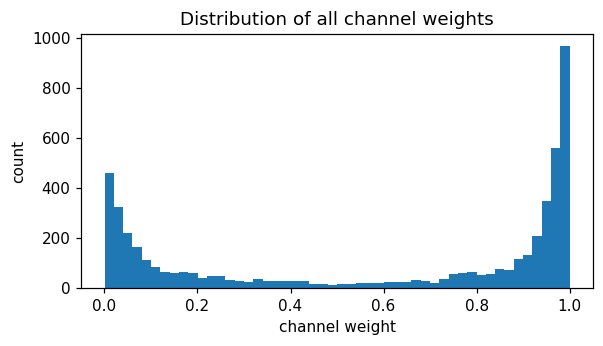
\includegraphics[width=0.45\linewidth]{13_channel_weight_hist.png}
\caption{Distribution of all channel weights.}
\end{figure}

The channel weights had a mean of $0.592$ and a standard deviation of
$0.407$, and $59.75\%$ of the weights were above $0.5$: the weights are
widely spread between small and large values rather than concentrated around
the mean, with many channels strongly weighted. The overlap (Jaccard index)
of the top-20 channels between different images was $0.75$, so a large
part of the favoured channels is the same for all images and the weighting
changes only moderately from image to image.

\subsection*{14.3 Spatial-Attention Visualization}

\begin{figure}[H]
\centering
\includegraphics[width=0.62\linewidth]{12_spatial_attention.eps}
\caption{Input, spatial attention map $M_s$ (Channel$\rightarrow$Spatial at $P_3$, resized to $224\times224$) and its overlay for the five test images (red = value near 1, blue = low value).}
\end{figure}

The spatial-attention values ranged from $0.403$ to $1.000$ with a mean of
$0.979$. The map is close to $1$ almost everywhere; the low-valued regions
are narrow areas along the image borders (mainly the bottom edge, and the
left or top edge in some images) and not the region around the flower or the
broad background. The module therefore does not segment the flower from the
background in this experiment.

\subsection*{14.4 Self-Attention Visualization}

\begin{figure}[H]
\centering
\includegraphics[width=0.8\linewidth]{13_self_attention.eps}
\caption{Self-attention at $P_3$: input, mean attention received, attention from the centre query position (star) and maximum attention received.}
\end{figure}

The learned scaling parameter was $\gamma=-0.0236$ and the attention matrix
had size $196\times196$ per image. The mean entropy of the attention rows was
$0.04$ nats, whereas a uniform distribution over $196$ positions has an
entropy of $5.28$ nats, i.e.\ the attention is extremely concentrated. In the
figure, the mean, the centre-query and the maximum attention maps are almost
identical for each image: all queries attend to one single location (a small
bright spot), whose position changes from image to image (for example on a
flower bud or flower in the tulip, rose and bouquet images, on a petal in the
close-up rose image and on a blurred background flower in the daisy image) but does not follow the position of the
query.

\subsection*{14.5 Attention at Different Depths}

\begin{figure}[H]
\centering
\includegraphics[width=0.78\linewidth]{14_attention_positions.eps}
\caption{Spatial-attention maps $M_s^{P_2}$ ($28\times28$), $M_s^{P_3}$ ($14\times14$) and $M_s^{P_4}$ ($7\times7$) of the three Channel$\rightarrow$Spatial models for the same five test images.}
\end{figure}

The statistics of the maps (mean / mean standard deviation over locations /
minimum / maximum) were: $P_2$: $0.967$ / $0.100$ / $0.150$ / $1.000$;
$P_3$: $0.979$ / $0.059$ / $0.403$ / $1.000$; $P_4$: $0.988$ / $0.052$ /
$0.168$ / $1.000$. At all three depths the map is near $1$ in most of the
image. At $P_2$ the low-valued areas are thin and finely structured along
the borders, with the largest variation over locations; at $P_3$ they are
larger blobs near the bottom (and left) edge; at $P_4$ they are single coarse
cells (the $7\times7$ grid) in the lower or background part of the image (for
example the lower-right of the first image and the left background of the
daisy image). At none of the depths do the low values fall on the flowers, so
the progression from edges to semantic flower regions that might be
expected was not observed in these maps.

% ============================================================
\section*{15. Qualitative Comparison}
% ============================================================

The same three correctly classified and two misclassified images were used
for all models.

\begin{figure}[H]
\centering
\includegraphics[width=\linewidth]{15_qualitative_main.eps}
\caption{Input, Grad-CAM of the baseline, Channel and Channel$\rightarrow$Spatial models, spatial-attention map (Spatial model) and mean self-attention received, all at $P_3$. Under each input: true class, baseline prediction and prediction of the selected model.}
\end{figure}

\textbf{Observations.} For the three correctly classified images (tulips,
daisy, roses) the Grad-CAM maps of the baseline, Channel and
Channel$\rightarrow$Spatial models are located on the same region: the red
flower heads, the daisy centre and petals, and the centre of the rose bouquet,
with the baseline and the attention models differing only slightly in extent.
For the misclassified tulips image (\texttt{test[476]}, predicted as roses by
both baseline and selected model) the baseline and Channel maps lie on the
centre of the bouquet, whereas the Channel$\rightarrow$Spatial map is
shifted to the left of the bouquet and covers a broader region. For
\texttt{test[507]} (true roses; baseline predicted tulips) the baseline
focuses on a spot in the lower right of the image, the Channel map is
spread over several spots, and the Channel$\rightarrow$Spatial map covers an
upper-left central region. The spatial-attention map of the Spatial model is
near $1$ over the image with low values in a strip along the top border for
all five images, and the self-attention response is a single small spot
that does not coincide consistently with the flower. Hence, the qualitative
differences between the models were largest for the incorrectly classified
images and small for the correctly classified ones; because only five images
were examined, no general conclusion is drawn from them.

\begin{figure}[H]
\centering
\includegraphics[width=\linewidth]{16_qualitative_extended.eps}
\caption{Grad-CAM of the baseline, SE (Channel), ECA, CBAM, Self-attention and CoordAtt at $P_3$ for the same five images.}
\end{figure}

For the three correctly classified images, ECA, SE and CBAM give maps on the
same flower region as the baseline, self-attention gives a broader map on the
rose bouquet, and CoordAtt gives broader, less peaked maps on all images
(consistent with its larger coverage, $0.330$ versus $0.189$, and lower
compactness, $0.429$ versus $0.560$, in Section 13). For the misclassified
images the mechanisms differ strongly from each other: for
\texttt{test[507]} the SE, ECA, self-attention and CoordAtt maps are located
in different parts of the image (CoordAtt over a large central area) and the
CBAM map has an additional hot spot in the bottom-left corner away from the
flower; for \texttt{test[476]} the CBAM map extends from the bouquet toward the
lower part of the image, whereas the other maps remain on the bouquet.

% ============================================================
\section*{16. Additional Attention-Mechanism Comparison}
% ============================================================

ECA, CBAM and Coordinate Attention were compared with the mechanisms
implemented in the laboratory, with the same ResNet50 backbone and at the
same position $P_3=\text{after conv4\_x}$. The Channel model is the SE
block.

\begin{center}

\resizebox{\textwidth}{!}{
\begin{tabular}{|l|c|c|c|c|c|c|}
\hline

\textbf{Attention}
&
\textbf{Accuracy}
&
\textbf{Precision}
&
\textbf{Recall}
&
\textbf{Macro F1}
&
\textbf{Parameters}
&
\textbf{Inference Time}
\\
\hline

No Attention
&
0.9274
&
0.9263
&
0.9315
&
0.9268
&
23,597,957
&
4.03 ms/img
\\
\hline

Channel / SE
&
0.9165
&
0.9133
&
0.9165
&
0.9141
&
23,730,117
&
4.06 ms/img
\\
\hline

Spatial Attention
&
0.9347
&
0.9349
&
0.9349
&
0.9347
&
23,598,056
&
4.07 ms/img
\\
\hline

ECA
&
0.9165
&
0.9177
&
0.9173
&
0.9150
&
23,597,962
&
4.05 ms/img
\\
\hline

CBAM
&
0.9365
&
0.9348
&
0.9401
&
0.9367
&
23,730,216
&
4.08 ms/img
\\
\hline

Self-Attention
&
0.9256
&
0.9246
&
0.9229
&
0.9233
&
24,908,678
&
4.26 ms/img
\\
\hline

Additional Mechanism: Coordinate Attention
&
0.9238
&
0.9226
&
0.9234
&
0.9228
&
23,698,469
&
4.08 ms/img
\\
\hline

\end{tabular}}
\end{center}

CBAM was the best of these mechanisms in macro F1 ($0.9367$) and tied with
Channel$\rightarrow$Spatial at $P_2$ in accuracy ($0.9365$), at $132{,}259$
added parameters; the 99-parameter Spatial module was almost as accurate
($0.9347$); ECA ($5$ parameters) and SE ($132{,}160$ parameters) both
scored $0.9165$; and the lightweight self-attention ($1.31$\,M parameters)
and Coordinate Attention ($100{,}512$ parameters) were below the baseline in
accuracy. A larger module did not give higher accuracy. The Grad-CAM
comparison of these mechanisms is given in Section 15, and the compactness
and coverage statistics in Section 13.

% ============================================================
\section*{17. Discussion}
% ============================================================

\textbf{Quantitative.} The highest test accuracy and macro F1 of all trained
models were obtained with the $5\times5$ spatial kernel ($0.9456$ / $0.9447$),
followed by the Combined model ($0.9383$ / $0.9382$), Channel$\rightarrow$Spatial
at $P_2$ and CBAM ($0.9365$ each) and the Spatial model ($0.9347$). The
baseline reached $0.9274$ / $0.9268$. The largest gain over the baseline
($+0.0181$) is smaller than the $\pm0.022$ 95\% confidence interval of the
baseline accuracy, and so is every other difference in Section 9; the
differences between the models are therefore not statistically clear with a
551-image test set and a single run per model. Channel (SE), ECA and
Channel$\rightarrow$Spatial at $P_1$ fell $0.0109$ below the baseline. At the
class level, the selected multi-position model improved daisy and dandelion
but lost F1 in tulips, roses and sunflowers (Section 12).

\textbf{Computational.} The modules add between $5$ (ECA) and $5.77$\,M
(Combined at $P_4$) parameters, but the accuracy was not related to the cost
(Spearman $\rho=+0.26$, $p=0.31$ between parameters and accuracy;
$\rho=+0.13$, $p=0.62$ between inference time and macro F1). Self-attention
($+1.31$\,M parameters, $+0.22$\,ms) was below the baseline, and the Combined
model ($+1.44$\,M, $+0.27$\,ms) gained $0.0109$ accuracy, while the
132\,k-parameter C$\rightarrow$S and CBAM modules, the 99-parameter spatial
module and the 33\,k-parameter C$\rightarrow$S module at $P_2$ cost at most
$0.05$\,ms per image and gave similar or better accuracy than the heavier
modules. A light module therefore provided comparable performance to the
heavier mechanisms in this experiment.

\textbf{Position.} Among the Channel$\rightarrow$Spatial models at $P_1$ to
$P_4$ the best accuracy was obtained at $P_2$ ($0.9365$) and the worst at
$P_1$ ($0.9165$) and $P_4$ ($0.9220$): intermediate features
($28\times28\times512$ and $14\times14\times1024$) were the most useful
insertion points, whereas the high-resolution early features ($56\times56$,
256 channels) and the coarse, semantically strong final features
($7\times7\times2048$) gave no benefit. Attention at several stages ($P_3{+}P_4$,
$P_2{+}P_3{+}P_4$) was not better than at the single best stages, the order
of channel and spatial attention made no difference ($0.9328$ for both), and
the kernel size gave a non-monotonic result ($k=3$: $0.9238$, $k=5$:
$0.9456$, $k=7$: $0.9328$).

\textbf{Qualitative.} The spatial-attention maps were almost uniform ($\approx1$)
with low values on image borders only, at all three depths, so they did not
suppress the background around the flower. The self-attention collapsed to a
single location per image (entropy $0.04$ nats; $\gamma=-0.0236$), which
explains why it contributed little. The Grad-CAM maps of the attention models
were located on the same flower regions as the baseline for correctly
classified images and differed mainly for the misclassified ones; the
compactness statistic increased slightly for Spatial, Channel$\rightarrow$Spatial,
SE and CBAM ($0.570$--$0.582$ versus $0.560$) and decreased for self-attention
and CoordAtt. These qualitative observations are consistent with the
quantitative ones: the attention modules changed the network only slightly
and no consistent advantage was found. An internal attention map shows what
the module re-weights, whereas Grad-CAM shows what drives the class score;
here the internal maps were nearly uniform, while Grad-CAM maps were
flower-centred for both the baseline and the attention models.

\textbf{Limitations.} A single seed per model, a small test set ($551$
images, $\pm2\%$ confidence interval), a short schedule ($5+5$ epochs), only
conv5\_x unfrozen, the $\gamma$-initialised self-attention (which starts as
an identity mapping), and hardware-dependent timings. Qualitative
conclusions are based on five (and, for Grad-CAM, ten) test images.

% ============================================================
\section*{18. Conclusion}
% ============================================================

Under a controlled protocol on a pretrained ResNet50 and the \texttt{tf\_flowers}
dataset, all 17 attention variants reached test accuracies between $0.9165$ and
$0.9456$ against $0.9274$ for the baseline, i.e.\ every change was inside the
confidence interval of a 551-image test set. The best results were obtained
with the $5\times5$-kernel Channel$\rightarrow$Spatial module at $P_3$
($0.9456$), Combined attention ($0.9383$), and Channel$\rightarrow$Spatial
attention at $P_2$ and CBAM ($0.9365$). Intermediate stages ($P_2$, $P_3$)
worked better than the earliest ($P_1$) and the last ($P_4$) stage, repeated
attention at several stages and a larger module (self-attention, Combined) did
not help, and the order of channel and spatial attention did not matter. Cost
did not predict performance, and the learned internal maps were nearly uniform
(spatial) or collapsed (self-attention). For this dataset and protocol, the
attention effectiveness therefore depended mostly on the position (feature
resolution and semantics) and much less on the type or the complexity of the
module; a firm ranking of mechanisms would need several seeds and a larger
test set.

% ============================================================
\section*{19. Answers to Required Questions}
% ============================================================

\begin{enumerate}\small

\item \textbf{Purpose of residual connections.} A block learns a residual $F(x)$ and outputs $F(x)+x$; the identity path gives gradients a direct route to earlier layers, which makes very deep networks trainable and avoids the degradation problem.

\item \textbf{conv2\_x versus conv5\_x.} conv2\_x is the first three bottleneck blocks ($56\times56\times256$; edges, textures, colours); conv5\_x is the last three ($7\times7\times2048$; large receptive field, class-level parts and objects).

\item \textbf{Why resolution decreases.} Stride-2 convolutions / max-pooling at the start of conv3\_x, conv4\_x and conv5\_x halve the resolution, growing the receptive field, reducing computation and memory and building translation invariance, at the cost of spatial detail.

\item \textbf{Why channels increase.} More filters are needed to represent the growing variety of abstract patterns; doubling the channels when halving each spatial side keeps the computation per stage roughly balanced.

\item \textbf{Low-, intermediate- and high-level features.} Low-level: edges, colour blobs, orientations; intermediate: repeated textures, petal arrangements and parts; high-level: whole-object, class-discriminative semantics.

\item \textbf{Purpose of attention.} To re-weight features adaptively (depending on the input), emphasising informative content and suppressing less useful content at small cost.

\item \textbf{Channel attention} learns \emph{what} is important: a vector $M_c\in\mathbb{R}^C$ of channel gates.

\item \textbf{Spatial attention} learns \emph{where}: a map $M_s\in\mathbb{R}^{H\times W}$ of important locations.

\item \textbf{Difference.} Channel attention is a global per-channel gate (spatially uniform); spatial attention is a per-location gate (channel-uniform).

\item \textbf{Sequential use.} They operate on different axes and are complementary, so they compose: select informative channels, then locate them (CBAM and the C$\rightarrow$S module).

\item \textbf{Channel attention at conv3\_x versus conv5\_x.} At conv3\_x the channels encode generic textures and parts shared by many classes, so the weights tend to be less selective; at conv5\_x the 2048 channels are close to class-specific detectors, so gating them is closer to a re-weighting of class evidence; the hidden widths also differ ($512/16=32$ versus $2048/16=128$). In the experiments, the channel weights were measured only at $P_3$ (Section 14.2), where they were widely spread (mean $0.592$, standard deviation $0.407$).

\item \textbf{Spatial attention at an intermediate stage.} At $28\times28$ or $14\times14$ the map has enough resolution to localise, while the features already carry part-level semantics, so a spatial gate could suppress clutter before the later stages; at $7\times7$ the grid is coarse. In the experiments the best result was at $P_2$ ($0.9365$), although the learned maps were nearly uniform.

\item \textbf{Cost of self-attention.} Its cost is $O(N^2d)$ in time and $O(N^2)$ in memory with $N=HW$.

\item \textbf{Size of the self-attention matrix.} It grows with the square of the number of positions: $2{,}401$ entries at $P_4$, $38{,}416$ at $P_3$, $614{,}656$ at $P_2$ and $9{,}834{,}496$ at $P_1$ per image ($37.52$\,MB in fp32); doubling each side of the feature map multiplies it by 16.

\item \textbf{Effect of the position on performance.} For Channel$\rightarrow$Spatial attention the accuracy was $0.9165$ ($P_1$), $0.9365$ ($P_2$), $0.9328$ ($P_3$) and $0.9220$ ($P_4$) versus $0.9274$ for the baseline: only $P_2$ and $P_3$ were above the baseline, and all differences were within the confidence interval.

\item \textbf{Attention at $P_2$ versus $P_4$ visually.} The $P_2$ map ($28\times28$) has thin, finely structured low-valued areas along the borders (standard deviation over locations $0.100$, minimum $0.150$); the $P_4$ map ($7\times7$) has coarse single-cell low-valued areas (standard deviation $0.052$, minimum $0.168$); both are $\approx1$ elsewhere (mean $0.967$ versus $0.988$) (Section 14.5).

\item \textbf{Does attention at multiple stages always help?} No: $P_3{+}P_4$ gave $0.9238$ and $P_2{+}P_3{+}P_4$ gave $0.9292$, compared with $0.9328$ at $P_3$ alone and $0.9365$ at $P_2$ alone, while adding $658{,}822$ and $692{,}233$ parameters.

\item \textbf{Channel$\rightarrow$Spatial versus Spatial$\rightarrow$Channel.} Accuracy was identical ($0.9328$) and macro F1 was $0.9323$ versus $0.9313$; no meaningful difference was found.

\item \textbf{Influence of the spatial kernel size.} The accuracy for $k=3,5,7$ was $0.9238$, $0.9456$ and $0.9328$ (macro F1 $0.9243$, $0.9447$, $0.9323$); the dependence was non-monotonic and the cost nearly the same. The maps for $k=3$ and $k=5$ were not visualised.

\item \textbf{SE versus ECA.} SE uses two fully connected layers with a bottleneck (reduction $r$), so every channel interacts with all others after a dimensionality reduction; ECA removes the reduction and applies a 1-D convolution of adaptive kernel size over the pooled vector (local cross-channel interaction, only $k$ parameters: $5$ at $P_3$ versus $132{,}160$ for SE).

\item \textbf{CBAM} applies channel attention (average- and max-pooled descriptors through a shared MLP, summed, sigmoid) and then spatial attention (channel-wise average and max maps, $7\times7$ convolution, sigmoid), sequentially.

\item \textbf{Self-attention versus channel attention.} Channel attention gives one scalar gate per channel from pooled statistics, with no interaction between positions; self-attention computes content-dependent pairwise affinities between all positions ($N\times N$) and mixes their values, so each location uses information from distant locations.

\item \textbf{Does the module with the most parameters give the highest accuracy?} No: Combined ($1.44$\,M added parameters) gave $0.9383$ and self-attention ($1.31$\,M) gave $0.9256$ (below the baseline), whereas the $5\times5$-kernel C$\rightarrow$S module ($132$\,k) gave the highest accuracy ($0.9456$) and ECA ($5$ parameters) gave $0.9165$ (Spearman $\rho=+0.26$, $p=0.31$).

\item \textbf{Internal attention map versus Grad-CAM.} An internal attention map is computed and used by the network in its forward pass (it changes the output); Grad-CAM is computed from activations and gradients of a trained model for a chosen class, does not alter the network, and is available with or without attention.

\item \textbf{Why Grad-CAM is post-hoc.} It is produced after training and prediction by back-propagating the class score, not as part of the model's computation.

\item \textbf{Does attention suppress irrelevant background?} Only marginally: the spatial maps were $\approx1$ except at the borders, and the Grad-CAM compactness changed from $0.560$ (baseline) to $0.570$--$0.582$ for Spatial, C$\rightarrow$S, SE and CBAM, with similar coverage, while self-attention and CoordAtt gave more diffuse maps.

\item \textbf{Attention maps for correct versus incorrect images.} The Grad-CAM maps of the attention and baseline models were similar for the three correctly classified images and differed mainly for the two misclassified ones (shifted, broader or multi-spot maps; Section 15); the spatial-attention maps were similar for all five images. This is based on five images only.

\item \textbf{Classes that benefit most.} Daisy ($+0.0445$ F1) and dandelion ($+0.0177$) for the selected model; tulips ($-0.0385$), roses ($-0.0358$) and sunflowers ($-0.0090$) became worse.

\item \textbf{Confusion matrix versus accuracy.} It shows which classes are confused with which (error structure, class bias), e.g.\ the increase of tulips$\rightarrow$roses from $10$ to $17$ with nearly unchanged accuracy; accuracy alone hides this.

\item \textbf{Why macro F1.} It averages the per-class F1 (balance of precision and recall) with equal class weight, so it is not dominated by larger classes and exposes weak classes.

\item \textbf{Accuracy--complexity trade-off.} The accuracy gain must be weighed against added parameters, memory, compute and training time (e.g.\ $+1.44$\,M parameters for $+0.0109$ accuracy with the Combined model).

\item \textbf{F1--inference-time trade-off.} Whether the additional latency per image buys a meaningful gain in macro F1; here the correlation was $\rho=+0.13$ ($p=0.62$).

\item \textbf{Same split for every ablation.} So that the differences can be attributed to the model change and not to different train/validation/test samples.

\item \textbf{Same training protocol.} The optimizer, schedule, epochs, augmentation and seed all affect accuracy; if they differ, the effect of the attention module cannot be isolated.

\item \textbf{Conclusions from the Grad-CAM comparison.} For correctly classified images the baseline and attention models focus on the same flower regions; differences appear mainly for misclassified images and in compactness/coverage (small for most modules, larger for self-attention and CoordAtt); the Grad-CAM evidence does not show a consistent improvement from attention, which agrees with the small, statistically unclear differences in accuracy.

\end{enumerate}

% ============================================================
\section*{20. References}
% ============================================================

\begin{enumerate}

\item
K. He, X. Zhang, S. Ren, and J. Sun,
``Deep Residual Learning for Image Recognition,''
\textit{Proceedings of the IEEE Conference on Computer Vision and Pattern
Recognition (CVPR)}, pp. 770--778, 2016.

\item
J. Hu, L. Shen, S. Albanie, G. Sun, and E. Wu,
``Squeeze-and-Excitation Networks,''
\textit{IEEE Transactions on Pattern Analysis and Machine Intelligence},
vol. 42, no. 8, pp. 2011--2023, 2020.

\item
S. Woo, J. Park, J.-Y. Lee, and I. S. Kweon,
``CBAM: Convolutional Block Attention Module,''
\textit{Proceedings of the European Conference on Computer Vision (ECCV)},
pp. 3--19, 2018.

\item
Q. Wang, B. Wu, P. Zhu, P. Li, W. Zuo, and Q. Hu,
``ECA-Net: Efficient Channel Attention for Deep Convolutional Neural
Networks,''
\textit{Proceedings of the IEEE/CVF Conference on Computer Vision and Pattern
Recognition (CVPR)}, pp. 11534--11542, 2020.

\item
Q. Hou, D. Zhou, and J. Feng,
``Coordinate Attention for Efficient Mobile Network Design,''
\textit{Proceedings of the IEEE/CVF Conference on Computer Vision and Pattern
Recognition (CVPR)}, pp. 13713--13722, 2021.

\item
A. Vaswani et al.,
``Attention Is All You Need,''
\textit{Advances in Neural Information Processing Systems},
vol. 30, 2017.

\item
R. R. Selvaraju, M. Cogswell, A. Das, R. Vedantam,
D. Parikh, and D. Batra,
``Grad-CAM: Visual Explanations from Deep Networks via
Gradient-Based Localization,''
\textit{Proceedings of the IEEE International Conference on Computer Vision
(ICCV)}, pp. 618--626, 2017.

\item
TensorFlow Documentation:
\url{https://www.tensorflow.org/}

\item
Keras Documentation:
\url{https://keras.io/}

\item
TensorFlow Datasets:
\url{https://www.tensorflow.org/datasets}

\end{enumerate}

\end{document}
